\documentclass{beamer}
\usetheme{metropolis}           % Use metropolis theme
\usepackage[german]{babel}  
\usepackage[utf8]{inputenc}	%dt Sonderzeichen wie ß
\usepackage{tikz}
\usepackage{amssymb}
\usepackage{multirow}
\usepackage{pgfpages}

%\setbeameroption{show notes on second screen=right}  %% Uncomment this to get Notes
\usetikzlibrary{arrows,positioning}

\renewcommand*{\figurename}{Abb.}




\title{Varianzanalyse - Teil II}
\date{22. Dezember 2016}
\author{Robert Feldhans}
\institute{Experimentelle Psychologie für Nichtpsychologen}
\begin{document}
	\maketitle
	
	\begin{frame}{Inhalt}
		\setbeamertemplate{section in toc}[sections numbered]
		\tableofcontents[hideallsubsections]
	\end{frame}
	
	\section{Interaktion}
	
	\begin{frame}{Rückblick}
		Interaktion
		\begin{itemize}
			\item zwischen mindestens zwei (signifikanten!) UV
			\item eingeteilt in verschiedene Klassen, abhängig von der Aussagekraft der UV
		\end{itemize}
	\end{frame}	
	
	\begin{frame}{Nullinteraktion - Diagramm}
		\begin{figure}
			\centering
			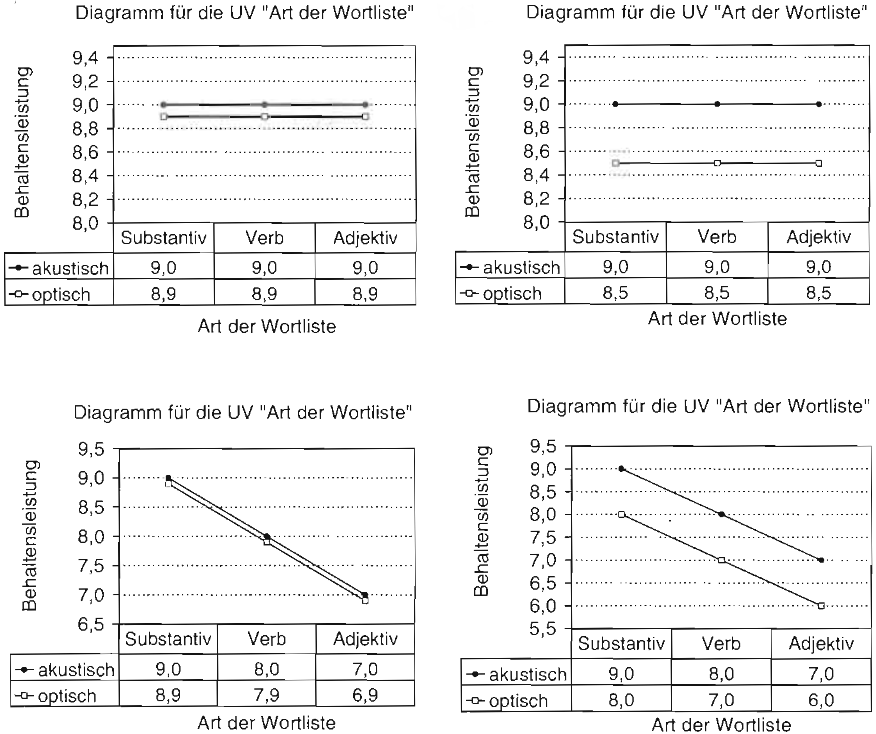
\includegraphics[width=0.8\textwidth]{Bilder/NullI.png}
		\end{figure}
		
		\note{
			\footnotesize
			Auf die unterschiedlichen Daten achten. Zellen zeigen. x-achse ist immer die betrachtete UV, über die wir eine aussage treffen wollen\\
			Bild mit vertauschten Achsen an die Tafel malen. Nachfragen, ob jemand Liniendiagramme noch nicht verstanden hat
			\begin{itemize}
				\item oben links: Unterschiedliche Ausprägungen der Faktorstufe haben gleiche Werte; keine Signifikanz\\ 
				\item oben rechts UV ``Präsentationsart'' unterscheidet sich von UV ``Wortart'' aber keine Abhängigkeit voneinander; keine Signifikanz bei der Wortart
				\item unten links Umgekehrter Fall zu oben rechts; keine Signifikanz bei der Präsentationsart
				\item unten rechts oben rechts und unten links kombiniert. Trotzdem parallel $\rightarrow$ keine Interaktion. Betrachtung der Daten legt ebenfalls nahe, dass keine Abhängigkeit besteht; Signifikanz bei beiden UV
			\end{itemize}
		}
	\end{frame}
	
	\begin{frame}{ordinale Interaktion - Diagramm}
		\begin{figure}
			\centering
			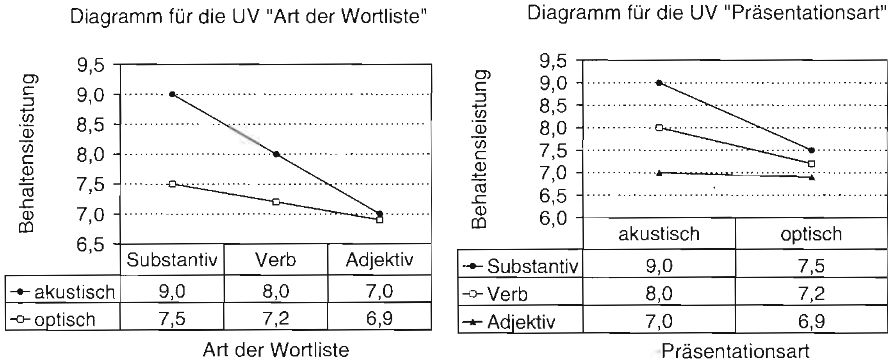
\includegraphics[width=1.0\textwidth]{Bilder/ordinaleI.png}
		\end{figure}
		\note{
			tatsächlich sind diese Diagramme eher unintuitiv, weil beide UV keiner ``echten Metrik'' folgen.\\
			Besseres Beispiel: Wir erheben die Größe von Personen anhand der Größe ihrer Eltern (UV1) und Kinder (UV2)\\
			Siehe Blatt.
		}
	\end{frame}
	
	\begin{frame}{disordinale Interaktion - Diagramm}
		\begin{figure}
			\centering
			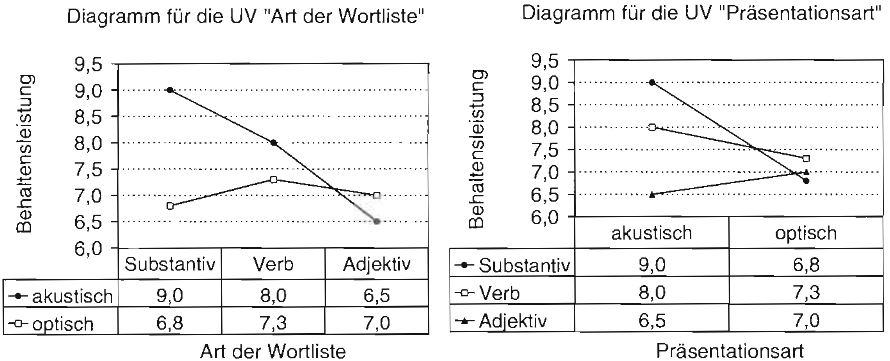
\includegraphics[width=1.0\textwidth]{Bilder/disordinaleI.png}
		\end{figure}
		\note{
			Was bedeuted das?\\
			Beim Durchgehen der Faktorstufen einen unabhängigen Variable mit einer speziellen Stufe der zweiten UV erhöht sich unsere abhängige Variable\\
			Beim durchgehen mit einer anderen Stufe der zweiten UV verringert sich jedoch unsere abhängige Variable\\
			$\rightarrow$ das gilt für beide diagramme/ achsenbelegungen!\\
			beispieldaten wären schöner gewesen, wenn die 7.0 eine 7.5 gewesen wäre, funktioniert aber trotzdem
		}
	\end{frame}
	
	\begin{frame}{semidisordinale Interaktion - Diagramm}
		\begin{figure}
			\centering
			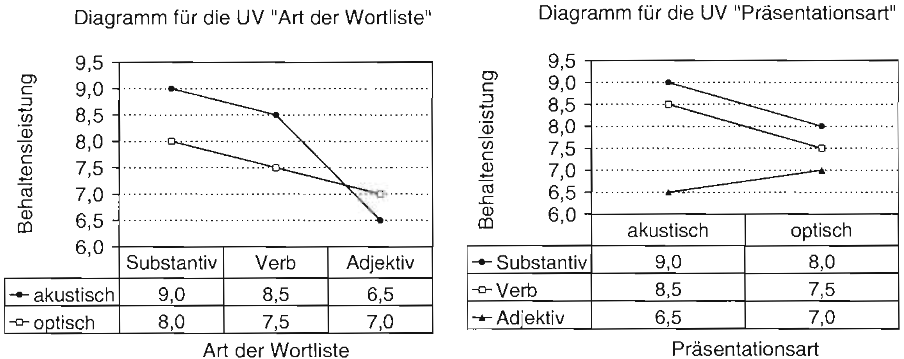
\includegraphics[width=1.0\textwidth]{Bilder/semidisordinaleI.png}
		\end{figure}
		\note{
			links: Kreuzen durch die adjektive, bei denen sich die reihenfolge umkehrt $\rightarrow$ dadurch kann keine Aussage für die Wortart getroffen werden (wir erinnern uns daran, dass bei der disordinalen I ebenfalls ein Wechsel auftrat)\\
			rechts: ordinale interaktion. tatsächlich sehen wir sogar eine art nullinteraktion (im bezug auf substantive und verben)\\
			kontraintuitive zuordnung von ``diagram für die uv x'' zu ordinalem faktor
		}
	\end{frame}
	
	\begin{frame}{Alternativdarstellung}
		\note{
			Unterschied zwischen der ursprünglichen und alternativen darstellung:\\
			ursprünglich: Kreuzen der Linien essentiell für disordinale Interaktion\\
			alternativ: (Aus-)Richtung der Linien essentiell, Überschneidung kann bei Disordi I vorkommen, muss aber nicht\\
		}
		Experiment
		\begin{itemize}
			\item Gesucht: Ursachen für Aggression
			\item Frust wird induziert, indem Probanden ein unlösbares Puzzle vorgelegt wird
			\item Kontrollgruppe mit lösbarem Puzzle
			\item als UV kommt die Raumtemperatur hinzu (20$^{\circ}$ bzw. 30$^{\circ}$)
		\end{itemize}
		Prinzip jetzt: Richtung der Linien
	\end{frame}
	
	\begin{frame}{Ordinale Interaktion alternativ}
		\begin{figure}
			\centering
			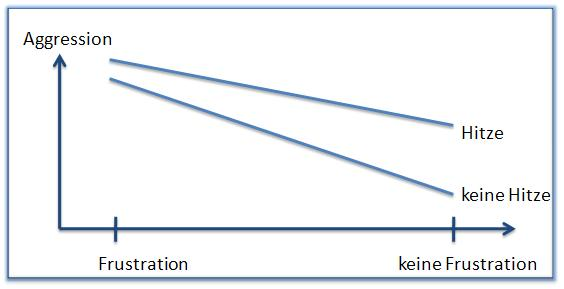
\includegraphics[width=0.6\textwidth]{Bilder/OrdinaleInteraktion1.jpg}
		\end{figure}
		\begin{figure}
			\centering
			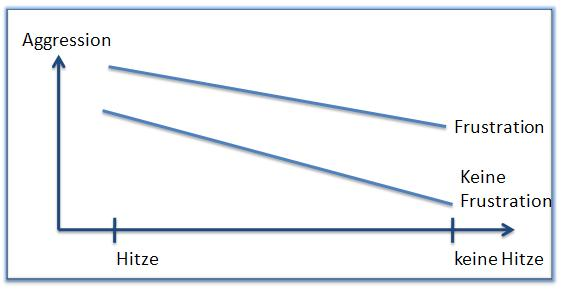
\includegraphics[width=0.6\textwidth]{Bilder/OrdinaleInteraktion2.jpg}
		\end{figure}
		\note{
			Bei der ordinalen Interaktion wird unsere Regel (Nicht-Kreuzen) erweitert\\
			Zusätzlich müssen sich beide Linien in dieselbe Richtung bewegen, z.b. sinken\\
			In diesem Beispiel: Der Wert von sowohl Hitze als auch keine Hitze muss von Frustration zu keine Frustration sinken\\
			Was sehen wir hier?\\
			Beide Achsendarstellungen der Versuchsergebnisse.\\
			Tritt auf bei ``spitzem Kegel''
		}
	\end{frame}
	
	
	\begin{frame}{Disordinale Interaktion alternativ}
		\begin{figure}
			\centering
			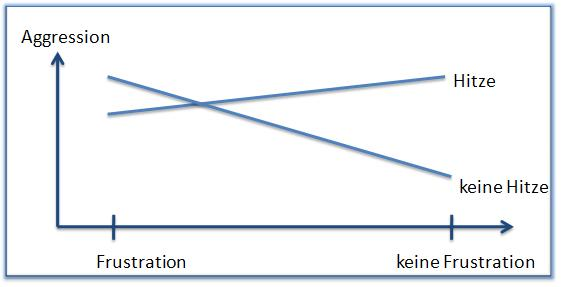
\includegraphics[width=0.6\textwidth]{Bilder/DisordinaleInteraktion1.jpg}
		\end{figure}
		\begin{figure}
			\centering
			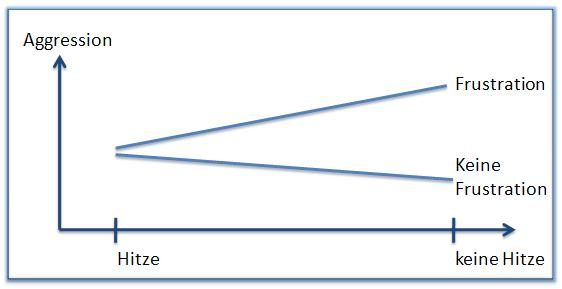
\includegraphics[width=0.6\textwidth]{Bilder/DisordinaleInteraktion2.jpg}
		\end{figure}
		\note{
			Bei der disordinalen Interaktion wird unsere Regel (Nicht-Kreuzen) verwässert\\
			kreuzen nur noch bei einem von beiden diagrammen notwendig
			tritt auf, wenn Richtung unterschiedlich und Kreuzen auftritt\\
			kann auftreten bei ``stumpfem Kegel''
		}
	\end{frame}
	
	
	\begin{frame}{Semidisordinale Interaktion alternativ}
		\begin{figure}
			\centering
			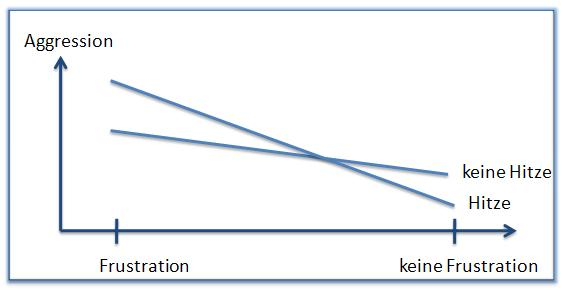
\includegraphics[width=0.6\textwidth]{Bilder/HybrideInteraktion1.jpg}
		\end{figure}
		\begin{figure}
			\centering
			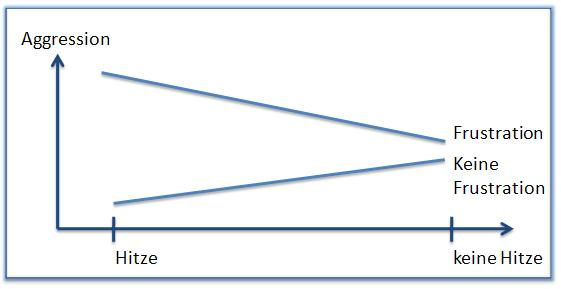
\includegraphics[width=0.6\textwidth]{Bilder/HybrideInteraktion2.jpg}
		\end{figure}
		\note{
			Tritt auf, wenn Richtung zwar gleich aber trotzdem Kreuzen auftritt\\
			Alternativ: ``Großer Kegel''
		}
	\end{frame}
	
	\begin{frame}{Interaktion alternativ - Zusammenfassung}
		\begin{itemize}
			\item Beide Linien zeigen in die selbe Richtung, ``spitzer Kegel''\\
			$\rightarrow$ ordinale Interaktion
			\item Kreuzen wegen unterschiedlicher Richtungen, ``stumpfer Kegel''\\
			$\rightarrow$ disordinale Interaktion
			\item Kreuzen trotz gleicher Richtungen, ``stumpfer Kegel''\\
			$\rightarrow$ semidisordinale Interaktion
		\end{itemize}
	\end{frame}
	
	\section{Anwendungsvoraussetzungen der Varianzanalyse}
	
	\begin{frame}{Allgemeine Voraussetzungen - Zufallsstichproben}
		\note{Zufallsstichprobe aus der Population werden in der Psychologie kaum verwendet $\rightarrow$ was bedeutet das für die Relevanz?\\}
		\begin{itemize}
			\item Die Qualität der Stichprobe ist wichtig für die Konstruktion der Stichprobenkennwerteverteilung \note{1. Stichprobenkennwerteverteilung geht von Zufallsstichprobe aus\\} \\
			$\rightarrow$ bildet Grundlage für die Signifikanzentscheidung
			\item Falls die Stichprobe nichtzufällig gezogen ist, konstruiert man eine hypothetische Grundgesamtheit \note{2. d.h. wir tuen einfach mal so, als wäre unsere Stichprobe repräsentativ\\}
			\item für diese gilt dann die entsprechende Stichprobenkennwerteverteilung, damit können wir unser Ergebniss gegen eine Zufallserklärung absichern\note{3. falls Signifikanz vorliegt\\}
			\note{Mal nen Bild dazu an die Tafel, Spuckspasti/ Anekdote zu Nutzerstudien/ }
		\end{itemize}
		\note{Diskussionsrunde: Welchen Wert haben die an Universitäten gefundenen Ergebnisse im Hinblick auf die Zufälligkeit der Stichprobe? Zitat: ``Im übrigen zeigt gerade die psychologische Forschung, dass es offensichtlich möglich ist, auch mithilfe nichtzufälliger Stichproben zu neuen Erkenntnissen zu gelangen, da praktisch nie mit echten Zufallsstichproben gearbeitet wird''}
	\end{frame}
	
	\begin{frame}{Allgemeine Voraussetzungen - Unabhängigkeit der Messungen}
		\begin{itemize}
			\item Der Einfluss von Störvariablen für jede Messung muss unabhängig sein vom Einfluss der Störvariablen jeder anderen Messung
			\item Das gilt sowohl innerhalb der, als auch zwischen den Stichproben
			\item d.h. insbesondere, dass es keine Subgruppen innerhalb der Stichproben geben darf
		\end{itemize}
		\note{
			\footnotesize
			Beispiel Hausaufgaben: Versuch, Ziel: beste Art der Hausaufgaben-Erteilung: kurzfristig (zb. jeden Tag die für den nächsten Tag) oder langfristig (am Ende des Monats müssen eine bestimmte Menge an Aufgaben erledigt sein, freie Zeiteinteilung)\\ Stichprobe aus zwei Klassen, die jeweils mit einer der Arten vertraut sind\\ Gemeinsame Vorerfahrung sorgt für abhängige Störvariablen\\
			Anderes Beispiel: Familienmitglieder in einer Studie, bei der Inividualdaten aufgenommen werden $\rightarrow$ Sozialer Background nicht unabhängig voneinander
			\begin{itemize}
				\item Der Einfluss von Störvariablen für jede Messung muss unabhängig sein vom Einfluss der Störvariablen jeder anderen Messung
				\item Das gilt sowohl innerhalb der, als auch zwischen den Stichproben
				\item d.h. insbesondere, dass es keine Subgruppen innerhalb der Stichproben geben darf
			\end{itemize}
		}
	\end{frame}
	
	\begin{frame}{Skalenniveau}
		\begin{itemize}
			\item Varianzanalyse macht nur Aussagen über Mittelwerte\\
			$\rightarrow$ sollte nur auf Daten angewendet werden, bei denen eine Aussage über Mittelwerte sinnvoll ist
			\item d.h. die erhobenen Daten sollten mindestens einer Metrik unterliegen
			\item \alert{allerdings:} Manchmal lässt sich aus einer sinnvollen Interpretation auch auf eine sinnvolle Anwendung ``Rückschließen''\\
			$\rightarrow$ bspw. Schulnoten
		\end{itemize}
		\note{
			\begin{itemize}
				\footnotesize
				\item Varianzanalyse macht nur Aussagen über Mittelwerte
				$\rightarrow$ sollte nur auf Daten angewendet werden, bei denen eine Aussage über Mittelwerte sinnvoll ist
				\item d.h. die erhobenen Daten sollten mindestens einer Metrik unterliegen
				\item \alert{allerdings:} Manchmal lässt sich aus einer sinnvollen Interpretation auch auf eine sinnvolle Anwendung ``Rückschließen'' \textbf{hier heiligt der swag die Mittel roflcopter}
				$\rightarrow$ bspw. Schulnoten\textbf{Schulnoten: Ist 1 doppelt so gut wie 2? 4x so gut wie 4? Noten in Prozent angeben $\rightarrow$ beim Programmieren: Erste 80\% der Anforderungen brauchen 20\% der Zeit, die nächsten 20\% 80\% der Zeit}
				\textbf{anmerken, dass für die VA die ursprüngliche Population natürlich auch normalverteilt sein muss, bei anderen Verteilungen macht die VA keinen Sinn}
			\end{itemize}
		}
	\end{frame}
	
	\section{Automatisches Berechnen mit Matlab und Python}%TODO komplett streichen?
	
	\begin{frame}{Varianzanalyse mit Matlab}
		\begin{itemize}
			\item stuff
			%% Fitte ein Model mit den eben bestimmten Faktoren und ihren Faktorstufen, welche den Vx entsprechen, welche Normalverteilt sind.
			
			rm = fitrm(data,'V1-V6~1','WithinDesign',factors);  % ~1: sind normalverteilt
			%data sind die daten; V1-V6 sind die Versichspersonen; 'withindesign' matlabmagic; factors ist ein muster, nach dem nachher die daten analysiert werden
			%fitrm = Fit repeated measures model
			
			%% Berechne Varianzanalyse für die Faktoren Wortart und Wiederholung sowie ihre Interaktion
			ranovatbl = ranova(rm,'WithinModel','Wortart * Wiederholung')
			%ranova = Repeated measures analysis of variance
		\end{itemize}
	\end{frame}
	
	
	\begin{frame}{Varianzanalyse mit Matlab - Beispiel}
		\begin{figure}
			\centering
			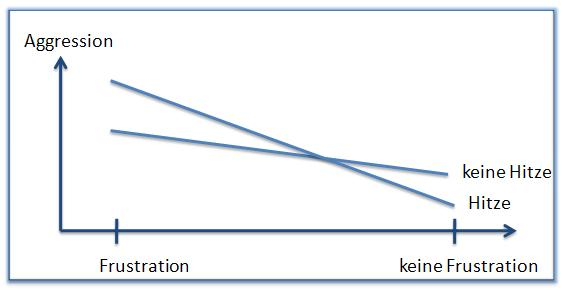
\includegraphics[width=0.6\textwidth]{Bilder/HybrideInteraktion1.jpg}
		\end{figure}
	\end{frame}
	
	
	\begin{frame}{Varianzanalyse mit Python}
		\begin{itemize}
			\item stuff
		\end{itemize}
	\end{frame}
	
	\begin{frame}{Varianzanalyse mit Python - Beipiel}
		\begin{figure}
			\centering
			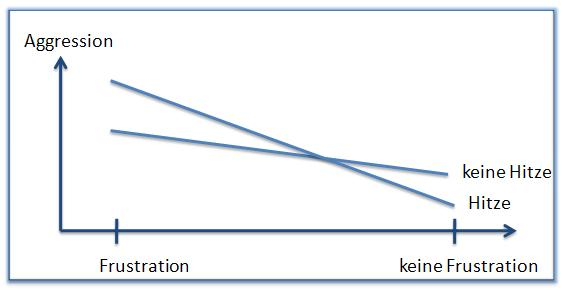
\includegraphics[width=0.6\textwidth]{Bilder/HybrideInteraktion1.jpg}
		\end{figure}
	\end{frame}
	
\end{document}

	